\section{Results}
\label{sec:results}

\todoMissing{update results with correct values}

%% --------------------------------------------

\subsection{Kernel Function}
\label{subsec:kernfunc}
The kernel function we ended up using for our final result was the following: 
\begin{equation}
k(s, \sigma) = k(5, 20) + k(10, 50) + k(100, 200) + ks(200, 500)
\end{equation}
where $s$ is the scaling.

%% --------------------------------------------

\subsection{Kernel Model}
\autoref{fig:kernel_model} shows mean of the the kernel model we generated with the above kernel.
\begin{figure}
	\centering
  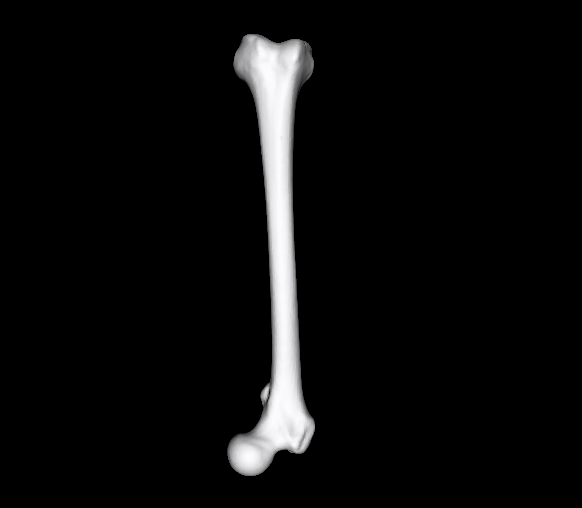
\includegraphics[scale=0.7]{./Figures/kernel_model}
  \caption{Mean of the kernel model.}
  \label{fig:kernel_model}
\end{figure}

%% --------------------------------------------

\subsection{Registrations}
\label{subsec:registrresults}
While in the end we are only interested in the distance between our reconstruction and the ground truth, we can also use the average distance and the Hausdorff distance as an indication of how closely we were able to fit our kernel model to the training data. 
In contrast to the previous distances, we are able to calculate these ourselves and hopefully, a better representation of our training data also leads to a better reconstruction of the partial bones. 

We provided a part of these values in \autoref{tbl:example_registration_distance}. For the full table please refer to the appendix.

\begin{table}
\centering
\caption{Example distances from fitted model to training data}
\label{tbl:example_registration_distance}
\begin{tabular}{lrr}
\toprule
\textbf{Bones} &
Average Distance &
Hausdorff Distance \\
\midrule
Bone 1& 0.3 & 2 \\
Bone 2& 0.3 & 2 \\
Bone 3& 0.3 & 2 \\
Bone 4& 0.3 & 2 \\
Bone 5& 0.3 & 2 \\
Bone 6& 0.3 & 2 \\
Bone 7& 0.3 & 2 \\
Bone 8& 0.3 & 2 \\
Bone 9& 0.3 & 2 \\
Bone 10& 0.3 & 2 \\
\bottomrule
\end{tabular}
\end{table}

\iffalse
\begin{table}
\centering
\caption{Distances from fitted model to training data}
\label{tbl:registration_distance}
\begin{tabular}{lrr}
\toprule
\textbf{Bones} &
Average Distance &
Hausdorff Distance \\
\midrule
Bone 1& 0.3 & 2 \\
Bone 2& 0.3 & 2 \\
Bone 3& 0.3 & 2 \\
Bone 4& 0.3 & 2 \\
Bone 5& 0.3 & 2 \\
Bone 6& 0.3 & 2 \\
Bone 7& 0.3 & 2 \\
Bone 8& 0.3 & 2 \\
Bone 9& 0.3 & 2 \\
Bone 10& 0.3 & 2 \\
Bone 11& 0.3 & 2 \\
Bone 12& 0.3 & 2 \\
Bone 13& 0.3 & 2 \\
Bone 14& 0.3 & 2 \\
Bone 15& 0.3 & 2 \\
Bone 16& 0.3 & 2 \\
Bone 17& 0.3 & 2 \\
Bone 18& 0.3 & 2 \\
Bone 19& 0.3 & 2 \\
Bone 20& 0.3 & 2 \\
Bone 21& 0.3 & 2 \\
Bone 22& 0.3 & 2 \\
Bone 23& 0.3 & 2 \\
Bone 24& 0.3 & 2 \\
Bone 25& 0.3 & 2 \\
Bone 26& 0.3 & 2 \\
Bone 27& 0.3 & 2 \\
Bone 28& 0.3 & 2 \\
Bone 29& 0.3 & 2 \\
Bone 30& 0.3 & 2 \\
Bone 31& 0.3 & 2 \\
Bone 32& 0.3 & 2 \\
Bone 33& 0.3 & 2 \\
Bone 34& 0.3 & 2 \\
Bone 35& 0.3 & 2 \\
Bone 36& 0.3 & 2 \\
Bone 37& 0.3 & 2 \\
Bone 38& 0.3 & 2 \\
Bone 39& 0.3 & 2 \\
Bone 40& 0.3 & 2 \\
Bone 41& 0.3 & 2 \\
Bone 42& 0.3 & 2 \\
Bone 43& 0.3 & 2 \\
Bone 44& 0.3 & 2 \\
Bone 45& 0.3 & 2 \\
Bone 46& 0.3 & 2 \\
Bone 47& 0.3 & 2 \\
Bone 48& 0.3 & 2 \\
Bone 49& 0.3 & 2 \\
Bone 50& 0.3 & 2 \\
\bottomrule
\end{tabular}
\end{table}
\fi

In \autoref{fig:registration_fit} you can see an example of the kernel model fitted to the training data.

\begin{figure}
	\centering
  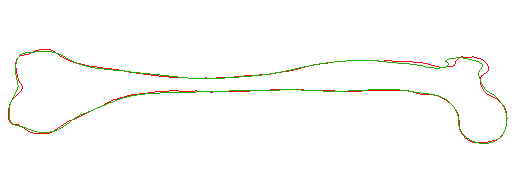
\includegraphics[scale=0.7]{./Figures/registration_fit}
  \caption{Example registration of the model to a bone from the training data}
  \label{fig:registration_fit}
\end{figure}

%% --------------------------------------------

\subsection{Trained Model}
\label{subsec:trainedmodel}
\autoref{fig:trained_model} shows the trained model we generated after fitting our kernel model to the training data.

\begin{figure}
	\centering
  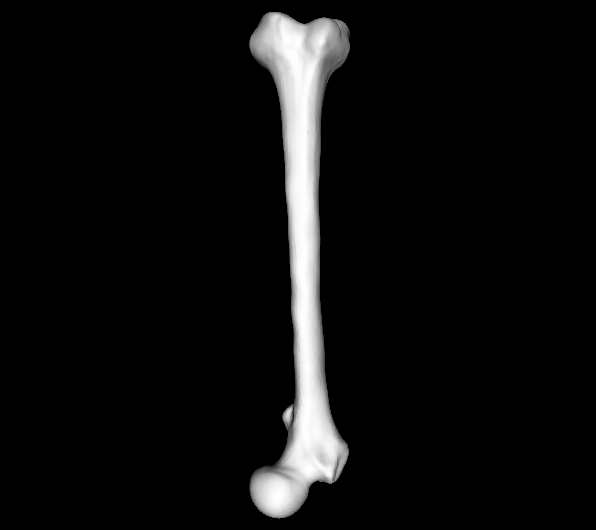
\includegraphics[scale=0.7]{./Figures/trained_model}
  \caption{Mean of the trained model.}
  \label{fig:trained_model}
\end{figure}

%% --------------------------------------------

\subsection{Reconstruction of Partial Bones}
\label{subsec:reconresults}
For the evaluation of the reconstruction of the partial bones, we are interested in closely modelling the actual bone, meaning we want our reconstruction and the ground truth data (not given to us) to be as close as possible. 
This will be tested using both the average distance and the Hausdorff distance between both meshes, both of which should ideally be as small as possible.

\autoref{fig:reconstructed_bone} shows a partial bone next to its reconstruction.

\begin{figure}
	\centering
  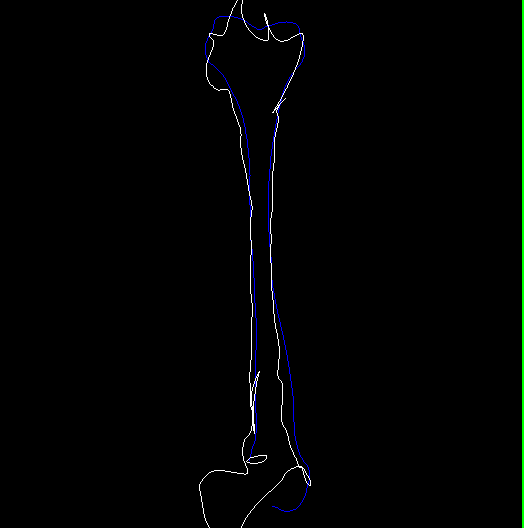
\includegraphics[scale=0.7]{./Figures/reconstructed_bone}
  \caption{Example reconstruction of a partial bone.}
  \label{fig:reconstructed_bone}
\end{figure}

All ten images of the partial femur bones that were given alongside our reconstruction can be found in the appendix. 
Their average distance and Hausdorff distance scores can be found in \autoref{tbl:reconstructed_distance}.

\begin{table}
\centering
\caption{Distances from reconstructed bone to ground truth.}
\label{tbl:reconstructed_distance}
\begin{tabular}{lrr}
\toprule
\textbf{Bones} &
Average Distance &
Hausdorff Distance \\
\midrule
Bone 1& 0.3 & 2 \\
Bone 2& 0.3 & 2 \\
Bone 3& 0.3 & 2 \\
Bone 4& 0.3 & 2 \\
Bone 5& 0.3 & 2 \\
Bone 6& 0.3 & 2 \\
Bone 7& 0.3 & 2 \\
Bone 8& 0.3 & 2 \\
Bone 9& 0.3 & 2 \\
Bone 10& 0.3 & 2 \\
\bottomrule
\end{tabular}
\end{table}